From the given information, 
\begin{align}
    \frac{AE}{EC} =  \frac{AD}{DB}&=\frac{1}{3}
\end{align}
and $\vec{D}$ divides AB in the ratio $1:3$ internally. $\vec{E}$ divides AE in the ratio $1:3$ internally.  Hence, 
\begin{align}
    \implies \vec{D} &=\frac{3\vec{A}+\vec{B}}{4}\\
    &=\myvec{\frac{13}{4}\\[2em]\frac{23}{4}}\\
    \vec{E} &=\frac{3\vec{A}+\vec{C}}{4}\\
    &=\myvec{\frac{19}{4}\\[2em]\frac{20}{4}}
\end{align}
\begin{align}
    \text{Area of } \triangle ABC &= \frac{1}{2}\norm{\brak{\vec{B-A}} \times \brak{\vec{C-A}}}\\
    &=\frac{1}{2}\norm{\myvec{-3\\-1}\times \myvec{3\\-4}}\\
        &=\frac{1}{2}\begin{vmatrix}
    -3&3\\
    -1&-4
    \end{vmatrix}\\
    &=\frac{1}{2}\sbrak{\brak{-3\times -4}-\brak{-1 \times 3}}\\
    &=\frac{15}{2}
\end{align}
\begin{align}
    \text{Area of } \triangle ADE &= \frac{1}{2}\norm{\brak{\vec{D-A}} \times \brak{\vec{E-A}}}\\
    &=\frac{1}{2}\norm{\myvec{\frac{-3}{4}\\[2em]\frac{-1}{4}}\times \myvec{\frac{3}{4}\\[2em]\frac{-4}{4}}}\\
    &=\frac{1}{2}\begin{vmatrix}
    \frac{-3}{4}&\frac{3}{4}\\[2em]
    \frac{-1}{4}&\frac{-4}{4}
    \end{vmatrix}\\
    &=\frac{1}{2}\sbrak{\brak{\frac{-3}{4}\times \frac{-4}{4}}-\brak{\frac{-1}{4} \times \frac{3}{4}}}\\
    &=\frac{15}{2\times16}
\end{align}
\begin{align}
    \frac{\text{area of } \triangle ADE}{\text{area of } \triangle ABC}=\frac{1}{16}
\end{align}
See Fig. \ref{aug/2/1plot}.
\begin{figure}[!h]
 \centering
 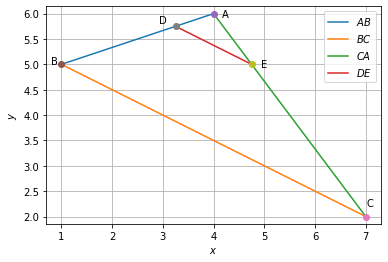
\includegraphics[width=\columnwidth]{solutions/aug/2/1/figs/figs.png}
 \caption{Plot of the triangles}
 \label{aug/2/1plot}
\end{figure}


